\pdfmapfile{+univers}%
\pdfmapfile{+dinbold}%
\documentclass[ngerman]{beamer}
\usepackage[utf8]{inputenc}
\usepackage[T1]{fontenc}
\usepackage[ngerman]{babel}
\usepackage{graphicx}
\usepackage{svg}
\usetheme[pagenum,nosectionnum,noheader,transition=push,headline=light]{tud}
\begin{document}
\title{FoodShip Group Update}
\subtitle{FoodShip, a foodsharing App}
\author{Sönke Huster \& Hannes Hilbert}
\date{\today}

\maketitle

  %  \frame{\frametitle{Inhaltsverzeichnis}\tableofcontents}

\section{Scenario}
\subsection{App Idea}
\frame{\frametitle{App Idea}
    \begin{itemize}
        \item App proposes having dinner with users nearby and a recipe based on the groups fridge content
    \end{itemize}
    \begin{figure}
        \begin{center}
            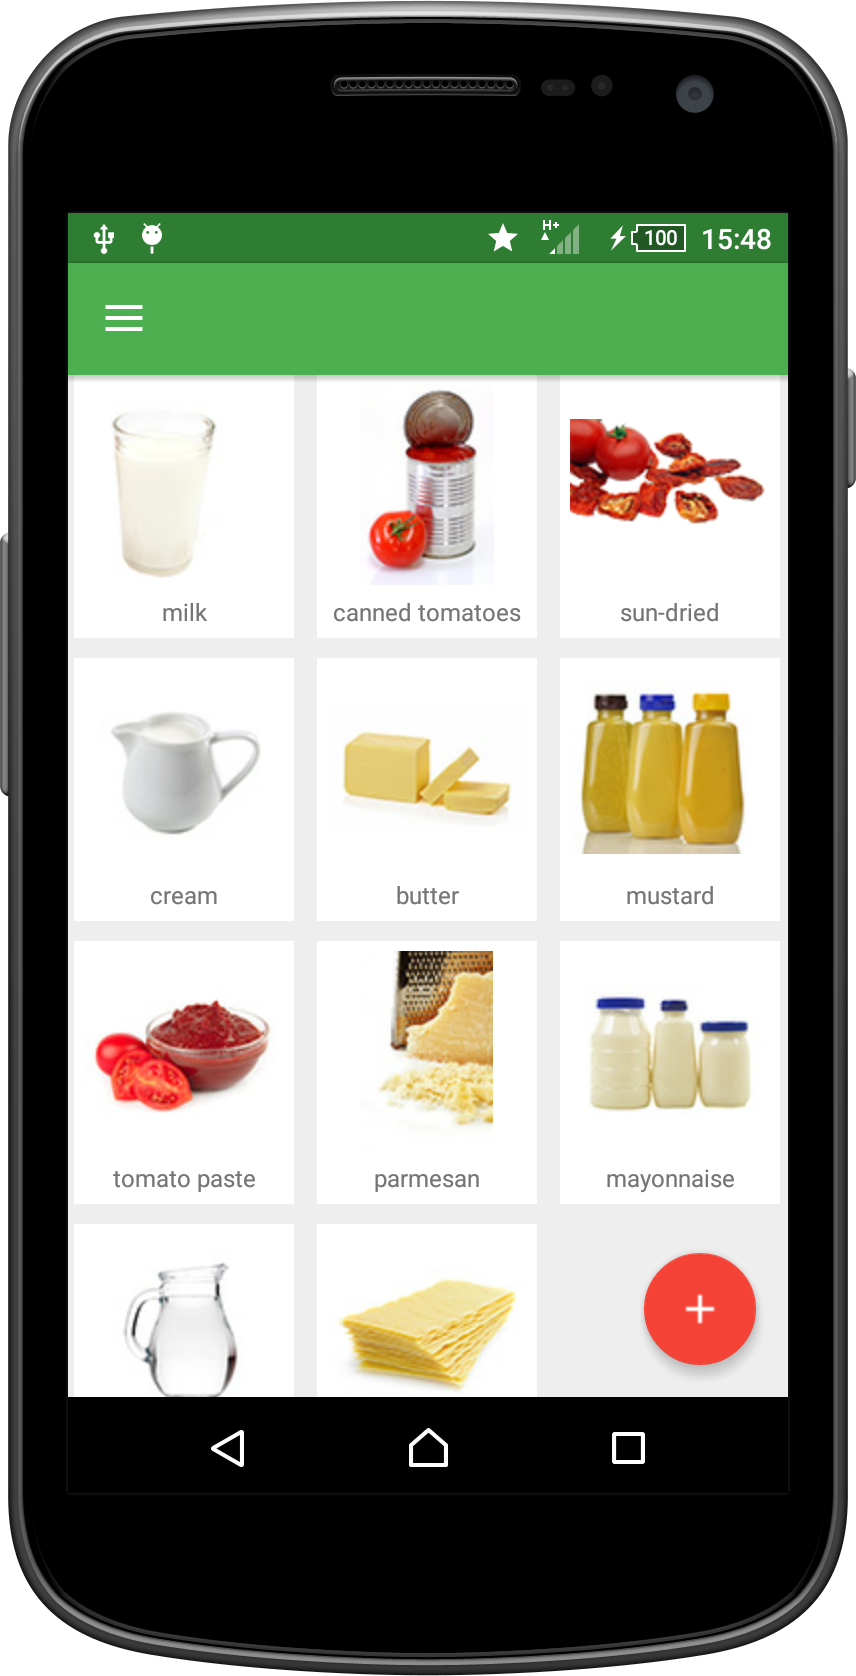
\includegraphics[width=0.25\textwidth,height=\textheight,keepaspectratio]{../screenshots/overview.png}
            \hspace{1cm}
            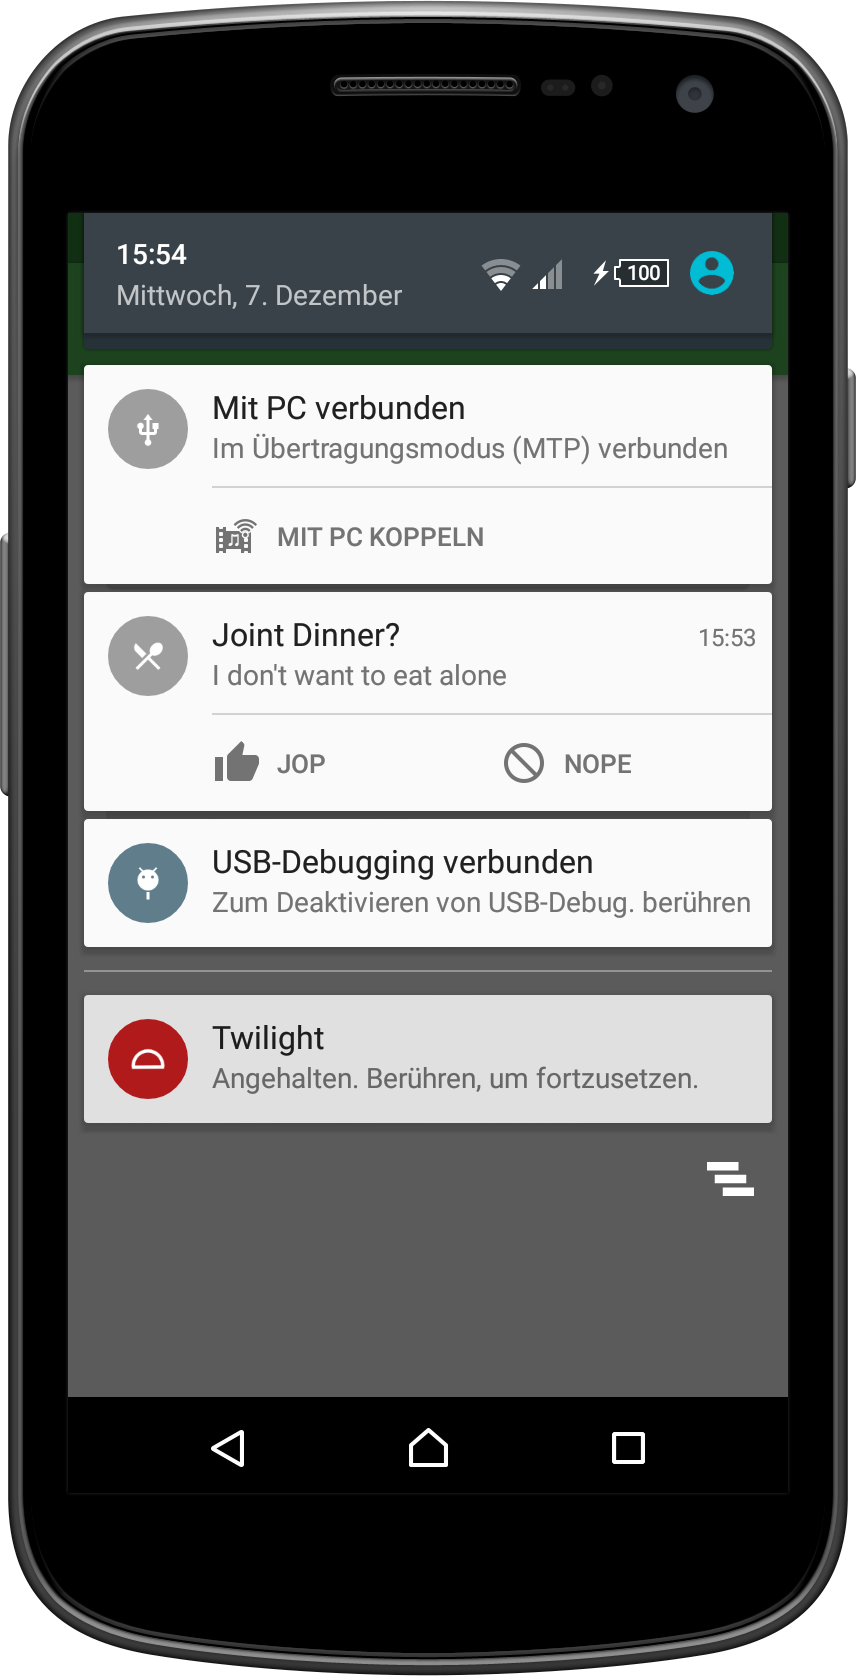
\includegraphics[width=0.25\textwidth,height=\textheight,keepaspectratio]{../screenshots/notification.png}
            \hspace{1cm}
            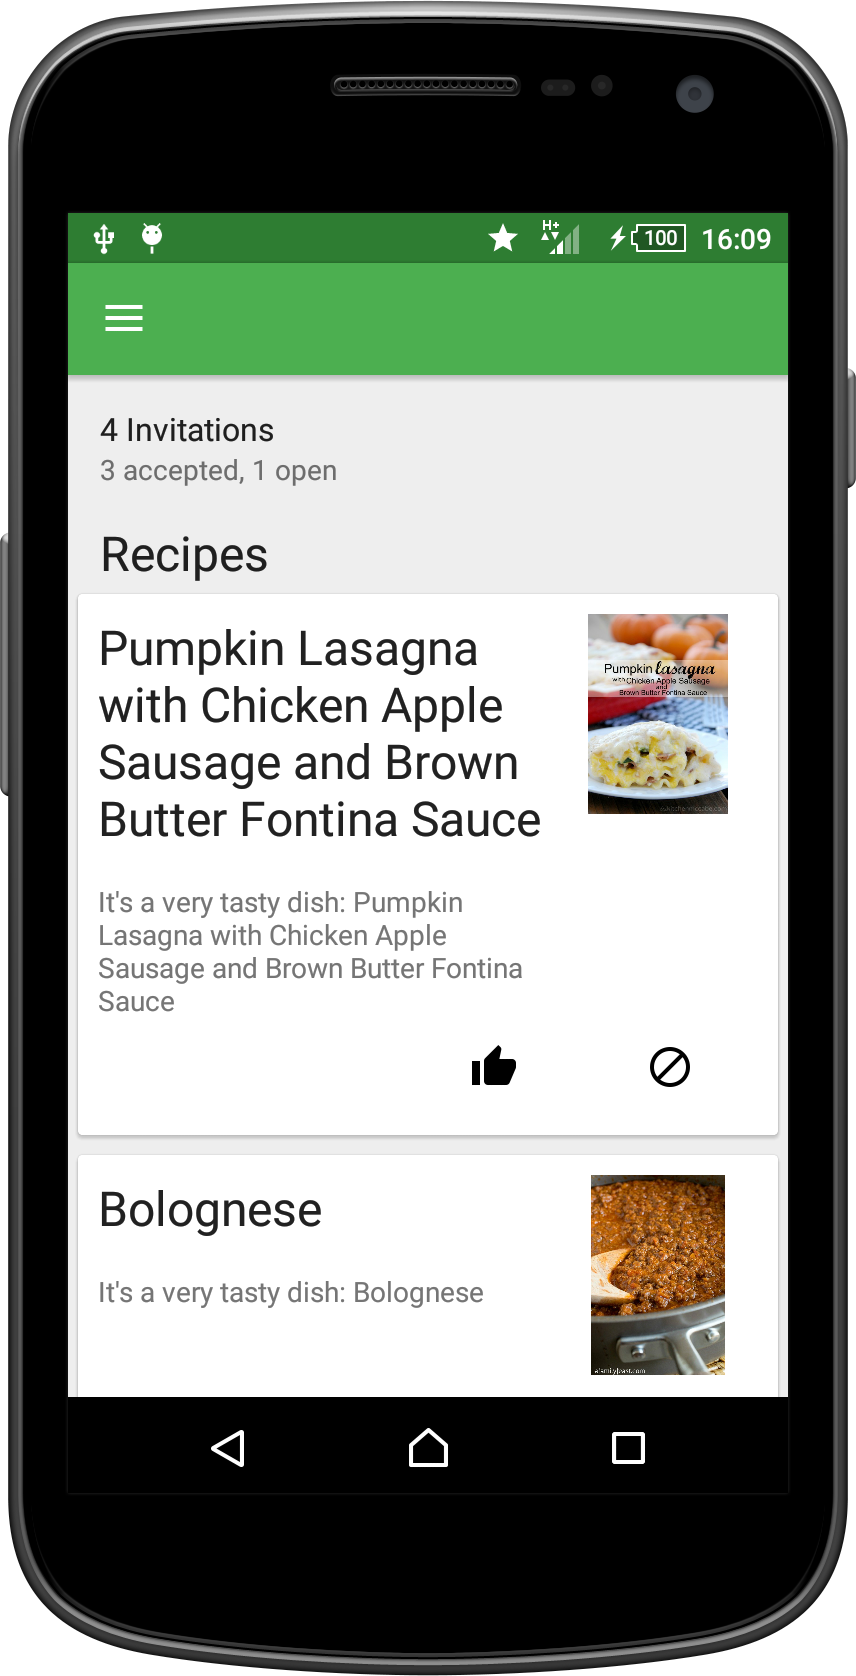
\includegraphics[width=0.25\textwidth,height=\textheight,keepaspectratio]{../screenshots/recipe_overview.png}
        \end{center}
    \end{figure}

}
\section{App Development}
\subsection{Architecture}
\frame{\frametitle{Architecture}
\begin{figure}
  \centering
  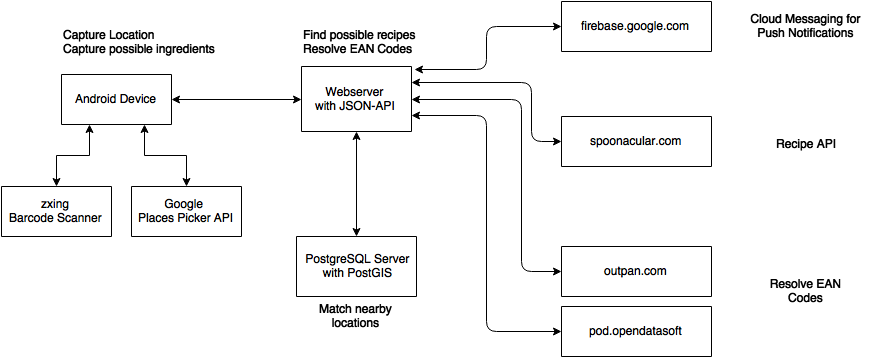
\includegraphics[width=0.9\textwidth,height=\textheight,keepaspectratio]{../diagrams/architecture_2.png}
\end{figure}
}

\section{Challenges}
\frame{\frametitle{Challenges \& Adaptation Concepts}

\begin{itemize}
\item  Connectivity challenge
\begin{itemize}
    \item Good looking recipes independent from connection type
\end{itemize}
\item  Offline Challenge
\begin{itemize}
    \item Keep recipes and dinner information while offline
    \item Add food while offline
\end{itemize}
\item  Energy Challenge
\begin{itemize}
    \item Keep invitations up to date
    \item Know the rough location
\end{itemize}
\end{itemize}
}
\frame{\frametitle{Ingredient adaptation}
    \begin{itemize}
        \item Suggest recipes that match many ingredients
        \item Example: Six of eleven ingredients needed for the best match
        \item Server regulary gets matching recipes
    \end{itemize}
    \begin{figure}
        \begin{center}
            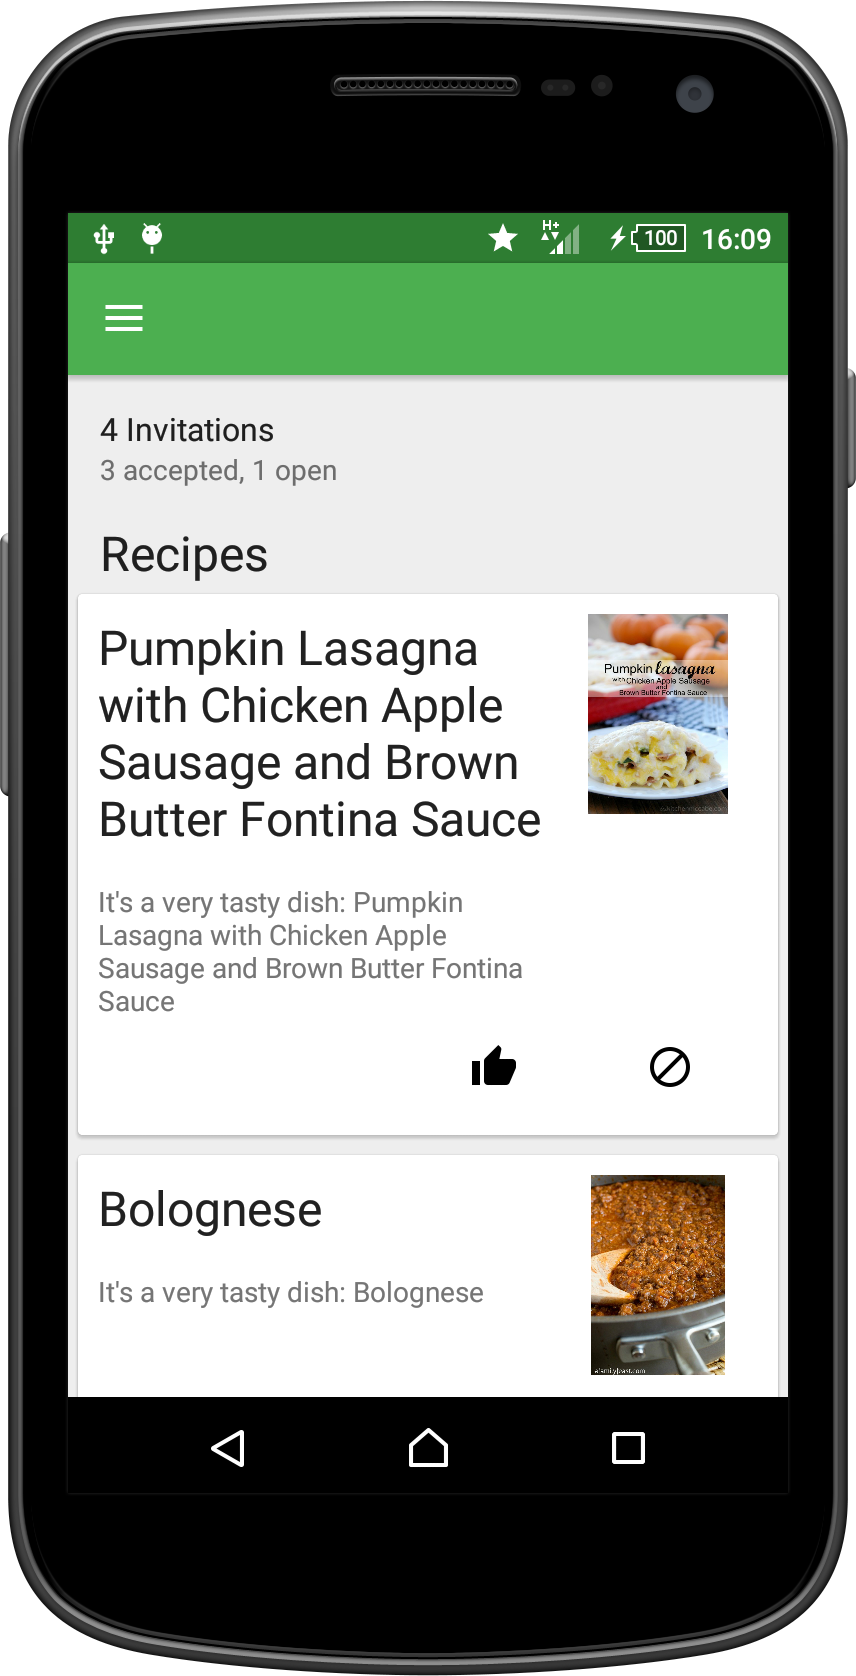
\includegraphics[width=0.2\textwidth,height=\textheight,keepaspectratio]{../screenshots/recipe_overview.png}
            \hspace{0.2cm}
            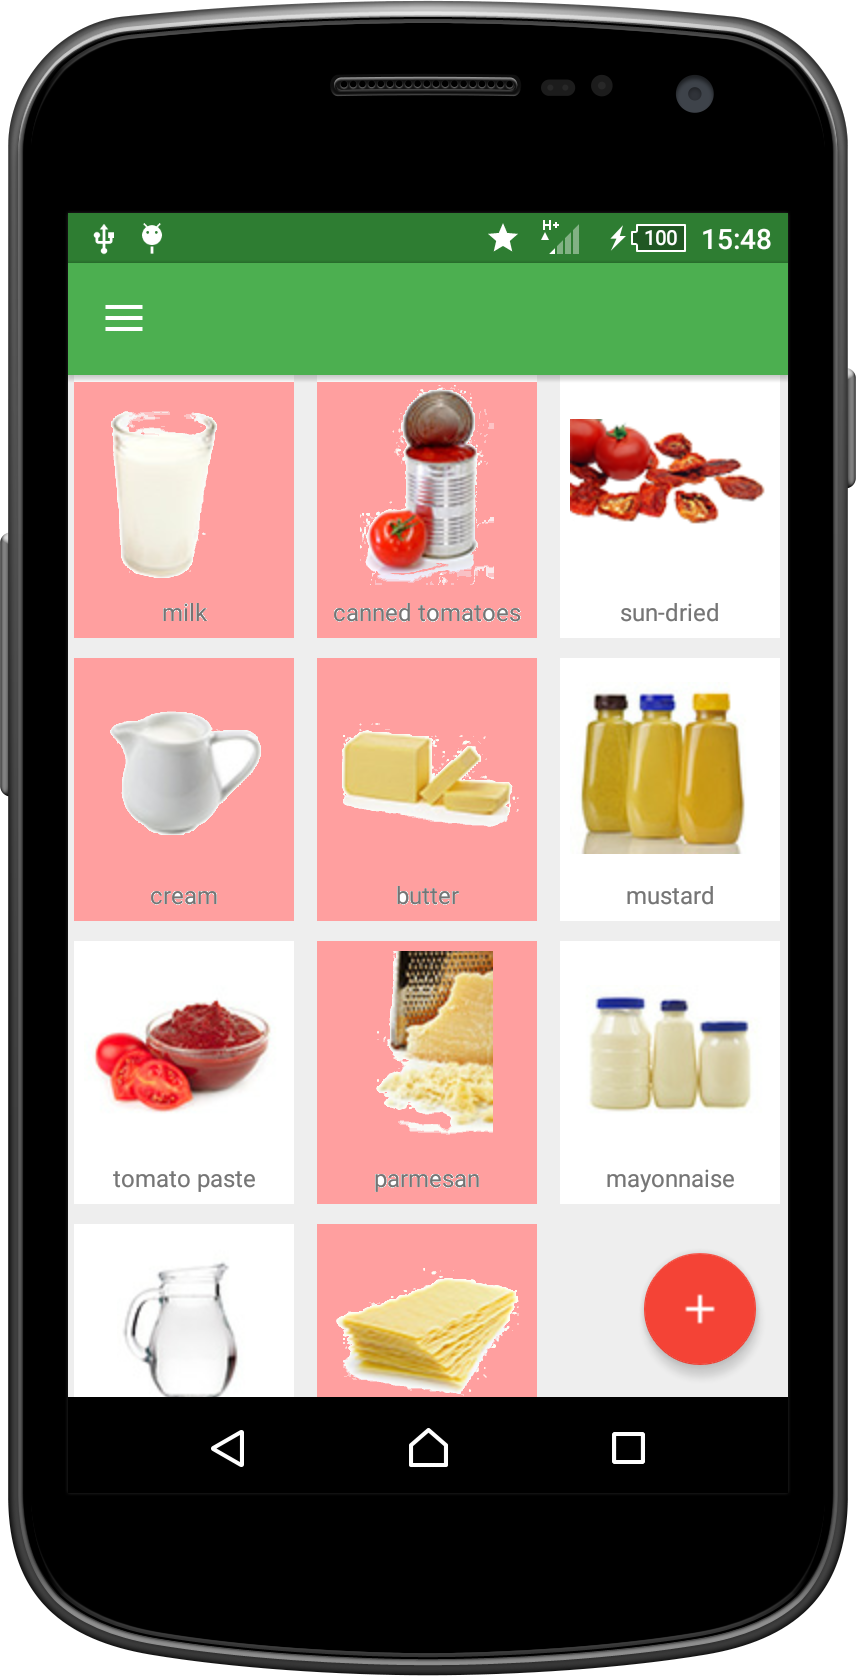
\includegraphics[width=0.2\textwidth,height=\textheight,keepaspectratio]{../screenshots/recipe_ingredients.png}
            \hspace{0.5cm}
            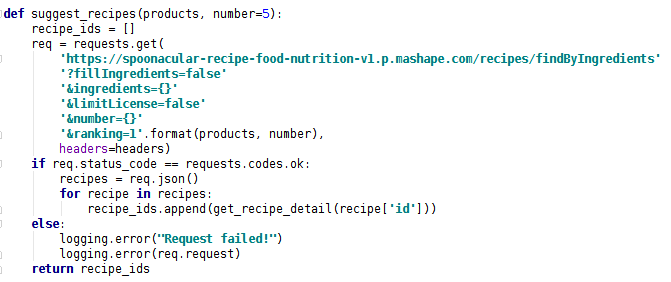
\includegraphics[width=0.5\textwidth,height=\textheight,keepaspectratio]{../screenshots/suggest_recipes_api_servercode.png}
        \end{center}
    \end{figure}
}
\frame{\frametitle{Location adaptation}
    \begin{itemize}
        \item Find groups of people nearby
        \item Server calculates groups by location
        \item Technology used: PostgreSQL Database with PostGIS Extension for location features
        \begin{itemize}
            \item PostGIS function example used in SQL Query: ST\_DISTANCE(user1.location, user2.location) < 1500
            \item Returns TRUE if user1 is in a 1.5km range of user2
        \end{itemize}
        \item Example: user\_id has X possible group\_members in a range of max\_distance
    \end{itemize}
    \begin{figure}
        \begin{center}
            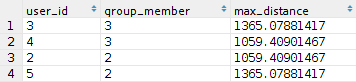
\includegraphics[width=0.4\textwidth,height=\textheight,keepaspectratio]{../screenshots/group_sql.png}
        \end{center}
    \end{figure}
}

\section{Prefetching}
\frame{\frametitle{Prefetching}
\vspace{0.4cm}
\begin{itemize}
  \item Push Notification triggered by our Server
  \item App prefetches Group informations and Recipe Pictures
  \item Data is persisted in internal Storage and in Cache for better User Experience
\end{itemize}
\begin{figure}
  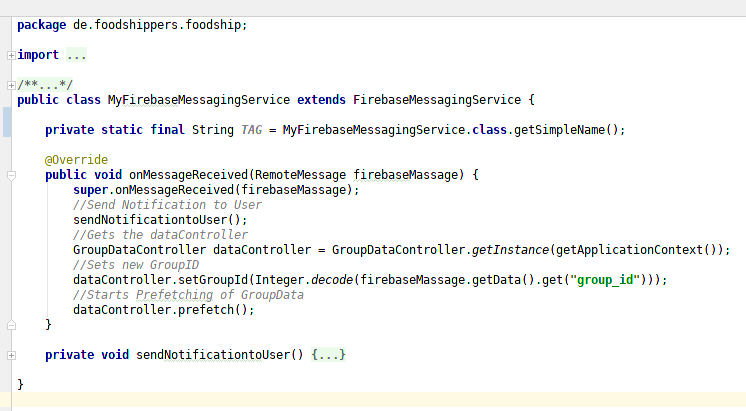
\includegraphics[width=0.8\textwidth,height=\textheight,keepaspectratio]{../screenshots/prefetching.png}
\end{figure}

}
\subsection{Workplan}
\frame{\frametitle{Workplan}
\begin{itemize}
  \item 16.12.2016 Second presentation
  \item 13.01.2016 End of implementation
  \item 27.01.2016 Third presentation
\end{itemize}
}
\end{document}
